\section{Depression}
\subsection{Bipolar Disorder}

Bipolar disorder is a disorder where a person experiences extreme mood swings. One day the person can feel amazing, and everything is fine, 
but the next day they feel like they do not belong anywhere in this universe. In general, one should be concerned about mood swings. 
It is, however, the extreme cases where the mind turns 180 degrees from day to day that is the main symptom of bipolar disorder. 
There is not a specific type of people that get this; they can be of any age and any gender, but most people that suffer from it find out 
(by having an experience or episode) around age 25 \cite{bipolar_statistics}. 

When talking about bipolar disorder, we often separate between the states \emph{normal}, \emph{mania} and \emph{depression}. 
The last two are the states we usually talk about since a normal state is not that interesting. These two states are very different, 
but they have some similarities, for example sleeping problems. 

When a bipolar person is in a manic state, he/she may do things that they would never have intended doing, like spending much money on items they do 
not need or abusing drugs/alcohol. They may also feel excited or powerful \cite{bipolar_overview}. 

A bipolar patient is in a depressive state when he or she is in a bad mood swing. They can stop doing everything they usually like to do, 
and lie down in bed all day with no motivation to do anything useful. They may feel useless and that they do not belong here, 
or being guilty of something they may or may not have done. In some cases, depression may even end up with suicidality, 
where the person either spends much time thinking of death, or attempt suicide.

The frequency of these symptoms can vary. One year they can have these mood swings every day for several weeks at the time, and the next they get them less frequent, 
like once every month. We also separate between bipolar disorder type I and II, with the main difference being that the manic episodes are way 
more aggressive in type I \cite{bipolar_types}. Statistics say that bipolarity is genetically inheritable, with 23\% chance of getting a child with bipolar 
disorder if one parent is bipolar, and 66\% if both parents are \cite{bipolar_statistics}. 

\subsection{Depression Rating: MADRS} %https://www.researchgate.net/publication/224773098_A_New_Depression_Scale_Designed_to_be_Sensitive_to_Change
Montgomery-Åsberg Depression Rating Scale, or MADRS for short, is a rating system for telling how depressed a patient is. Stuart A. Montgomery and Marie Åsberg 
designed it in 1979, and it is more sensitive to changes than the Hamilton Rating Scale for Depression (HRS) for patients that go through antidepressant medication. 
The process for calculating a MADRS rating contains ten statements about the patient's behavior, where the topics are \cite{madrs_paper}:

\begin{itemize}
    \item Apparent sadness
    \item Reported sadness
    \item Inner tension
    \item Reduced sleep
    \item Reduced appetite
    \item Concentration difficulties
    \item Lassitude
    \item Inability to feel
    \item Pessimistic thoughts
    \item Suicidal thoughts
\end{itemize}

The person doing the rating answers each question with a number between 0 and 6, where the higher the number, the more relevant the statement is for the patient. 
The numbers added together gives us the total MADRS score, which we split into four categories: normal/not depressed: 0-6, mild depression: 7-19, moderate depression: 
20-34 and severe depression: 34-60 \cite{sunnybrook_stroke_study}. 

\newpage
\section{Machine learning}
Machine learning is the field of computer science where we throw data into an algorithm and expect it to give answers to whatever the goal is, 
with as little work as possible. The process of performing machine learning was not as simple in the early days of the technology, 
but nowadays it is a lot easier with all the different frameworks and tools available.

Machine learning is a tremendous and almost magical technology, but knowing how one should use it can be difficult without the experience. 
The amount of data needed to make an algorithm learn something makes it difficult to get started, and to be efficient when training the model on a large dataset, 
decent hardware is required. One can get away with using a CPU if they want to test machine learning on a small dataset, but if the goal is to build something useful, 
too much time is saved using a GPU. 

The reason why GPUs are so much better than CPUs on this specific task is that the design choices of a CPU are for flexibility and general computing workloads. 
The GPU, on the other hand, is designed to do simple arithmetic instructions over and over again (easy to parallelize). These design choices make GPUs a lot more 
efficient for machine learning, and especially for deep neural networks \cite{cpu_vs_gpu_ml}. Alternatively, if investing in a GPU is not the preferred choice, 
there are many cloud services available to us today where we can pay a small sum in order to use a system that is a better fit for the task.

Now how do we make a machine learn? Well, there are many different approaches to this, which we will discuss in the next sections, but let us say we want to 
use a neural network for achieving some goal. Then our next step should be to choose a framework. We can, of course, do everything from scratch, but why 
reinvent the wheel when there are so many good frameworks and tools already out there? 

Python is a programming language perfect for machine learning in our opinion. The language looks a lot like pseudo-code, and this is perfect because we do not 
want to spend time on syntax rules in another language. A popular framework called \textbf{TensorFlow} is available to use in Python, and developers from Google have built it. 

TensorFlow allows the programmer to build models quickly, and also execute the training and testing. Before we get started with TensorFlow, a smart choice 
would be to do a quick search on the Internet to see if someone else has already done something similar to what we want to achieve, and if you find something, 
the odds are that your neural network model can be similar, if not identical to it. If not, then we have to sit down and write the model by ourselves. 

For the model implementation part, whether we found a model online or want to write it, we can, of course, use TensorFlow directly, but using \textbf{Keras} 
as an abstraction layer above TensorFlow is a popular choice. On their documentation website \cite{keras_docs}, they see their framework as 
\blockquote{A high-level neural networks API, written in Python and capable of running on top of TensorFlow, CNTK or Teano}.

Following their \textit{30 seconds to Keras} guide \cite{keras_docs}, you can create a \textit{sequential} model with \textit{dense}
layers, configure its learning process (compile), then fit, train, evaluate and predict with just a few lines of code \ref{code:keras-guide}.

\begin{code}
  \begin{minted}[linenos]{python}
      from keras.models import Sequential
      from keras.layers import Dense
  
      model = Sequential()
  
      model.add(Dense(units=64, activation='relu', input_dim=100))
      model.add(Dense(units=10, activation='softmax'))
  
      model.compile(loss='categorical_crossentropy',
                optimizer='sgd',
                metrics=['accuracy'])
      
      model.fit(x_train, y_train, epochs=5, batch_size=32)
      loss_and_metrics = model.evaluate(x_test, y_test, batch_size=128)
      classes = model.predict(x_test, batch_size=128)
  \end{minted}

  \caption{\textit{Simple introduction to Keras, where we create a Sequential model with two Dense layers, compile it with with the loss function Categorical Crossentropy and the optimizer SGD}}
  \label{code:keras-guide}
\end{code}


One thing that Keras does not make any easier is structuring the dataset so that the model can fit it. There is a high chance that we have to write some 
code ourselves to do this. Numpy is a package for Python built for math operations where everything happens optimally (Python by itself adds overhead to everything). 
All machine learning assumes that the input data is Numpy arrays, so experience with Numpy can be advantageous when structuring the dataset.

\section{Machine learning strategies}
Picking the right machine learning model can be quite tricky, especially if inexperienced. There are a couple of different \textit{strategies} one can choose 
from when deciding on a machine learning model. These are called \textit{supervised and unsupervised learning}, and we need to think about how the dataset is structured, 
and what we want to achieve to find out which one to use. The following sections will be a description of the strategies, to make the decision easier.

\subsection{Supervised learning}
Supervised learning is the machine learning strategy where we provide both input and correct output data to the algorithm \cite{supervised_learning_intro}. 
We may use supervised learning if the goal is to train a model to classify letters in the alphabet, or something else where we have a dataset with both input 
and output data (for the alphabet, images of letters are input data, and the actual letters are the output data). If we train this alphabet model, 
we will be able to input an image (not seen before by the algorithm) of a letter, and the model will classify it to the letter it most likely fits. 
This kind of supervised learning is called \textit{Classification} and is the problem of assigning new observations to the class they most likely belong, 
based on a classification model built from labeled training data \cite{machine_learning_for_humans_supervised_2}.

Another kind of supervised learning is called \textit{Regression} and is all about predicting (or estimating) a value. A classic example of regression 
learning is predicting income, using \textit{features} like home, location, job title, the field of study,  years of education and years of experience. 
We call these features \textit{categorical} (first three) and \textit{numerical} (last two) \cite{machine_learning_for_humans_supervised_1}. 

\subsection{Unsupervised learning}
Another strategy is unsupervised learning. We want to use this if we have a dataset without the same meaning as in a dataset for supervised learning. 
The items may not have a fixed answer, like the letters in the alphabet are. It is useful when we have unlabeled data and want to for example group data 
together in what we call a \textit{cluster}. Unsupervised learning may not be as common as supervised learning, but unsupervised learning can be quite 
beneficial in some cases; for example when grouping addresses together in neighborhoods if we have an unsorted list of addresses as the dataset.

\subsection{Semi-supervised learning}
Now, we may not always want to use one of the strategies above. Looking at the dataset, we may want something in between like a combination of labeled and unlabeled data. 
Semi-supervised learning comes in handy when this is the case. For example, if we have many data samples to label in our dataset, it can be simply too much work. 
We will not go deep into details about how this works, but it is important to mention it because of its usefulness.

\section{Machine learning approaches}
When we know whether we want to use supervised learning, unsupervised learning or something in between, we need to select an approach. We call them 
approaches because we use these regardless of the strategy that we end up using; most of them (except for reinforcement learning) work in both 
supervised and unsupervised learning. There are a lot of different approaches available, and we will describe some of them.

\subsection{Decision tree learning}
In computer science, trees are data structures commonly used to describe something that \textit{branches out} based on different input. For example, 
a tree can be a representation of how the frequency of letters in the alphabet are distributed in a text file so that the text file can be compressed optimally. 
We will not go into details about how this works, but our point is that tree-structures are very common in most fields of computer science. 

In machine learning, we can apply the tree-structures as \textit{decision tree learning}. In this approach, we set up all the different outcomes 
(with the training data set) of a specific question in a tree. Let us say we want to predict whether or not a person will run outside on a specific day. 
Then it makes sense that the training set contains weather information. The different data in the training set is called attributes, and correctly picking 
these is essential for the quality of the prediction.

\begin{table}
    \begin{tabular}{| l | l | l | l | l | l |}
    \hline
    \textbf{Day} & \textbf{Temperature} & \textbf{Outlook}   & \textbf{Humidity}  & \textbf{Wind}     & \textbf{Run} \\ \hline
            1    & 15 C                 & Sun                & Low                & Strong            & Yes \\
            2    & 6 C                  & Rain               & High               & Weak              & No  \\
            3    & 15 C                 & Rain               & Medium             & Strong            & Yes \\
            4    & 6 C                  & Overcast           & High               & Medium            & Yes \\
            5    & 15 C                 & Sun                & Low                & Weak              & No  \\
            6    & 12 C                 & Overcast           & Medium             & Weak              & No  \\
            7    & 12 C                 & Sun                & Medium             & Medium            & Yes \\
    \hline
    \end{tabular}
    \caption{Example training data set: days a person went out for a run}
    \label{table:days_running}
\end{table}

Table \ref{table:days_running} contains data about whether a person went outside for a run or not for a week (just an example, not real data). 
Here the first 4 (excluding "Day") columns (Temperature, Outlook, Humidity, and Wind) is the "predictors" and the last column (Run) is the target. 
To use this table in decision tree learning, we need to view it as a tree, with one of the predictors as the root node and the targets as leaf nodes. 

How we choose the tree structure is critical to the performance of the machine learning, and we need to use a good tree building algorithm. 
The most common algorithm to use in this situation is the \textit{ID3} algorithm made by J. R. Quinlan. It is a top-down, greedy search through the space 
of possible branches with no backtracking \cite{decision_tree}. The way this happens is by calculating \textit{Entropy} and \textit{Information Gain}. 
The idea is to recursively choose the predictor that has the highest information gain and generate a tree structure. With an optimal tree, 
we can create decision rules by merely following the tree with new data.

\subsubsection{Random Forest}
One known problem with decision tree models is that they often include much \textit{variance}. Variance in an algorithm means that it is sensitive to small 
changes in the training set. One method to reduce the variance is to use Random Forest. 

Random Forest is a supervised machine learning strategy, which can be useful for both classification and regression learning \cite{random_forest}. 
It mainly works by combining decision trees, where the tree building algorithm is heavily randomized for all trees. 

For example, if we want to get movie recommendations using machine learning, using one decision tree will most likely be insufficient. 
Just think what happens when we ask a friend for movies to watch. What that friend recommends is purely based on movies we like ourselves and what the friend likes. 
We might be lucky and find our next favorite movie, but most likely, asking multiple people for recommendations is going to yield better results. 
The same goes for machine learning, and decision trees will most likely give a better answer if we combine them in a Random Forest.

\subsection{Neural networks}

\subsubsection{General idea}
The general idea of machine learning with neural networks is to make the computer think like a human, inspired by the way biological neural networks in the human 
brain process information \cite{neural_networks_0}. There are a lot of different neural networks, but all of them share the same underlying layer-based architecture, 
where data get passed between layers where computation happens. The first layer is the input layer, which passes the data to the next layer, which is the hidden layers. 
The number of hidden layers is entirely up to the model and the programmer, and this is where the intermediate processing/computation is done before the data get passed 
to the output layer where we perform an activation function to define the output \cite{neural_networks_1}.

\begin{figure}[h]
    \begin{center}
        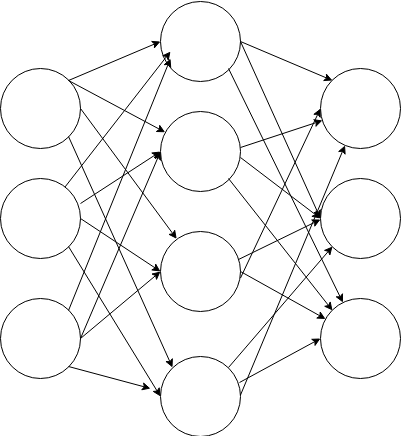
\includegraphics[height=10cm]{neural_net.png}
        \caption{Neural network visualization. The inputs on the left side are passed into the neurons in the hidden layer in the middle, which passes the values to the output layer.}
        \label{figure:neural_net}
    \end{center}
\end{figure}

If we have a lot of hidden layers in a neural network, we call it a \textit{deep} neural network. Deep networks can be useful for anything, and only the programmer's creativity sets the limit. Two common ways to use neural networks are \textit{Recurrent Neural Networks} and \textit{Convolutional Neural Networks}. These two have their use cases, which we will describe below.

Figure \ref{figure:neural_net} is a visual representation of a shallow neural network with the input layer on the left, one hidden layer in the middle and the output layer on the right-hand side. For each layer, we have fully connected nodes, which means that each node has a connection to all nodes in the next layer.

\subsubsection{Recurrent Neural Networks (RNN)}
This type of neural network is useful for predicting something based on a sequence of data, like for example predicting words in a sentence, which can be especially useful for typing on the phone. Also making predictions based on historical data, like a forecast, is something an RNN can do effectively.

One downside to Recurrent Neural Networks used on large sequences of data is that the prediction will most likely be off if a word written at the beginning of a long text is a dependency for a prediction four chapters later, for example, the home location of the main character. The workaround for this is something called \textit{Long Short-Term Memory Recurrent Neural Network (LSTM RNN)}, and is the idea of having additional logic to avoid the prediction model forgetting essential facts.

\subsubsection{Convolutional Neural Networks (CNN)}
A Convolutional Neural Network, or \textit{CNN} for short, can be used for identifying patterns in data, which then is the underlying calculations for either prediction or classification. A common use case for CNN's is image recognition. In image recognition, we train our models to be good at identifying objects in images, for example, the difference between cats and dogs. Then we can input a completely different image to the model, and it will output whether the image is of a cat or a dog. 

This type of CNN is two-dimensional because an input image is a two-dimensional array of pixels, so the network also needs to have two dimensions in the convolutional layers. Another way of constructing a CNN is one-dimensionally, which can be useful for \textit{one-dimensional} data, for example, sensor data from gyroscopes or accelerometers \cite{1d_cnn}.

\section{How can machine learning help people with bipolar disorder?}
The use of machine learning in the medical fields is growing exponentially. There is no limit to the usefulness of machine learning, and it can certainly help in the medical/psychological field too. Let us say bipolar patients had a device that measured their heart rate among other things 24 hours a day could feed the data into a neural network that gave the user's bipolar state as output. That would be useful for both the patients and doctors/nurses. Another use case could be if medical institutions knew in advance how many new bipolar patients to expect the next day. 

Using machine learning in this field of study could help many people get through their depression or mania, and potentially get rid of the condition altogether.

\section{Related work}

\subsection{Mental Health}
In the field of Mental Health Monitoring Systems (MHMS), research has already been done by many. In this section, we will describe a few papers that are of importance to this thesis, namely those about depression/bipolar disorder, who also applied machine learning to their study. 

E. Garcia-Ceja et al. surveyed some of the recent research works in machine learning for MHMS \cite{GarciaCeja2018_survey}. They gave the different works labels: study type (association/detection/forecasting), study duration (short-term or long term), and sensor types (wearable/external/software or social media). 

Association studies were those who help understand the relationships between variables, and the methods include linear regression, correlation analysis, t-tests and analysis of variance. Detection studies have a goal to detect/recognize mental state, often using methods like classification models. Forecast studies aim to predict events about patients, for example, epileptic seizures. The wearable sensor types include smart-watches and smartphones, external sensors could, for example, be cameras or microphones installed in an institution where the participants were patients. Some studies, where the sensor type was software or social media used services like Instagram to collect their data \cite{GarciaCeja2018_survey}. 

To find relevant work for this thesis, we had a look into some of the studies included, which studied depression and bipolar disorder. One study by O'Brien, J.T. et al. was an association study about depression, where the participants wore accelerometers on their wrists. Twenty-nine adults with depression and 30 healthy adults participated, and the goal was to study the possibility that physical activity has an impact on depression (referred to as Late Life Depressions in the paper). They found that the physical activity of participants with LLDs was significantly lower \cite{obrien_depression}, which is highly relevant for this thesis because our dataset contains physical activity data. 

Grünerbl, A. et al. had a detection type study about bipolar disorder. The participants consisted of ten bipolar patients in Austria between 18 and 65 years old. In this study, the recorded data was phone calls and microphone data and achieved an average recognition accuracy of 76\% and precision and recall of over 97\% of bipolar state detection. They also used the accelerometer and GPS as input data and achieved a recognition accuracy of 70\% (accelerometer) and 80\% (GPS) \cite{grunerbl_smartphone_bipolar}.

In a study by Maxhuni, A. et al., they used the same participants as the previous example. The difference was that in addition to using accelerometer and microphone data, they introduced questionnaires to the participants. For the results, they applied different machine learning algorithms, and their best average accuracy was 85.57\% \cite{maxhuni2016}.

Faurholt-Jepsen, M. et al. had an association type study about bipolar disorder. The participants were 29 bipolar patients, and actions on their smartphones like daily usage, the number of incoming calls, the number of text messages sent and received. They found correlations between the mental state of the patients and the recorded information. \cite{faurholt_smartphone_bipolar}

Andrew G. et al. applied machine learning to photos posted on Instagram. They had 166 participants, who posted a total of 43,950 photos. By extracting statistical features using colors analysis, metadata and face detection, they achieved models that outperformed the average practitioner's success rate when diagnosing depression (70\% of all depressed cases identified) \cite{instagram_depression}. Research on social media usage in the field of mental health is interesting because, for many, those are the platforms that they use to express their feelings. 

Mowery, D. et al. did another study based on social media, but instead of Instagram, they used Twitter. For a tweet, they classified whether or not it contained evidence of depression, and there was evidence of depression, they classified one of three symptoms (mood, disturbed sleep or loss of energy). The features they extracted from each tweet included \textbf{syntax} (usage of first/third person pronouns), \textbf{emoticons} usage (happy/sad), and \textbf{sentiment} (whether the text was subjective/objective and positive/negative). They achieved the best performance when classifying that a tweet had no evidence of depression, and their other models performed significantly worse \cite{twitter_depression}. 

The authors of the paper mentioned first surveying different machine learning research in MHMS, Garcia-Ceja, E. et al., also released a paper on motor activity based classification of depression in unipolar/bipolar patients. They applied machine learning for classifying depressed/nondepressed participants using Random Forest and a deep neural network (DNN). The dataset is the same as we used here in this thesis (described in detail in the next chapter), and they achieved an F1-score of 0.73 with Random Forest and 0.7 with the DNN. Since one of our goals is to do the same classification as this paper, it worth mentioning.

\subsection{Convolutional Neural Networks}

In most of the papers previously mentioned, the complexity of the machine learning models has not been the area of focus, but rather comparing different simple algorithms like decision trees and Naïve Bayes. A study by Kiranyaz, S. et al. used a 1-d convolutional neural network on real-time patient-specific ECG (electrocardiogram) classification \cite{ecg_1d_conv}. While this paper is not in the field of mental health, we found exploring how others have created convolutional neural networks essential for us when building our models. 

Kiranyaz, S. et al. achieved superior classification performance comparing it to most of the state-of-the-art methods, and concluded with the fact that after training a CNN dedicated to a patient, it can be solely responsible for classifying their ECG records \cite{ecg_1d_conv}. 

Human activity recognition (HAR) is another field of study where machine learning has shown its value. Ronao, C. A. et al. presented a deep convolutional network for classifying human activity (walking, sitting, standing and laying) based on a 1-d time-series of measurements from smartphone sensors \cite{ronao_har_conv}. The accuracy they achieved on their test set (95.75\%) outperformed the previous state-of-the-art models. 

The usage of convolutional networks is, of course, not limited to the medical field. Ince, T. et al. published a paper on real-time motor fault detection using a 1-d CNN. They used raw signal data as input to the model, and a model that only has to be trained once for each motor they achieved an accuracy of detecting motor faults above 97\% \cite{motor_fault_conv}.